% !TEX root = ../../main.tex
\chapter{Systematic Uncertainties} 
\label{ch:syst}

In this chapter, the systematic uncertainties considered in this analysis are specified. In \Sect{\ref{ch:syst:exp_unc}}, experimental uncertainties related to physics objects are described. \Sect{\ref{ch:syst:bkg_unc}} outlines the systematic uncertainties related to background modeling.  In \Sect{\ref{ch:syst:sig_unc}}, the theoretical uncertainties related to signal modeling are explained. In the statistical analysis described in~\Ch{\ref{ch:stats}}, each systematic uncertainty is treated as a nuisance parameter (NP). Event yields for the background and signal samples are determined corresponding to varying the systematic uncertainties by $\pm 1\sigma$.

%%
\section{Experimental Uncertainties}
\label{ch:syst:exp_unc}
Experimental uncertainties related to reconstructed physics objects are considered.  These uncertainties can affect both the shape and the normalization of simulated background and signal distributions. 

%
\subsection{General Uncertainties}
The total integrated luminosity for the 2015 + 2016 dataset used in this analysis has a 3.2\,\% uncertainty, measured following the prescription in~\Ref{\cite{lumi_unc}}. A calibration of the luminosity scale was performed in August 2015 and May 2016 with $x-y$ beam separation scans. This uncertainty is applied to the scaled event yields of all generated MC samples.

Variation in the PU re-weighting of MC is included to cover the uncertainty on the ratio between the predicted and measured inelastic cross section in the fiducial volume defined by $M_X>13\, \GeV$, where $M_X$ is the mass of the hadronic system~\cite{prw_unc}. The variation in re-weighting is applied to all generated MC samples. 

%
\subsection{Leptons}
Uncertainties for reconstructed leptons have a minor impact on this analysis. Uncertainties are considered for trigger efficiencies, reconstruction and identification efficiencies, isolation efficiencies, and determination of the momentum scale and resolution~\cite{electron_efficiency_2016, muon_eff}. For muons, the uncertainty on the \MET trigger efficiency is considered, including efficiency differences between \ttbar and \Wjets MC samples. The rest of the uncertainties are estimated using data and MC samples corresponding to $Z\ra \ell^+\ell-$ and $J/\Psi\ra\ell^+\ell^-$ resonances, with a tag and probe method where isolated leptons are used to tag the event. The estimated uncertainties depend on both $\eta$ and $\pT$. They are propagated and applied to the scale factors used to correct the simulated MC samples. The uncertainty on the electron (muon) reconstruction and identification efficiencies is $<0.5\,\%$ ($<1.0\,\%$). For muons, this includes an uncertainty corresponding to the efficiency of the track to vertex association. For both types of leptons, the isolation efficiency has an associated uncertainty below $1\,\%$. The momentum scale and momentum resolution have approximate uncertainties of $0.5\,\%$ ($0.05\,\%$) and $1\,\%$ ($2\,\%$) for electrons (muons), respectively. The uncertainty applied to the muon momentum scale includes charge-dependent effects.  

%
\subsection{Small-R Jets}

For small-R jets, uncertainties are included to account for the efficiency of the jet vertex tagger (JVT), the jet energy scale and resolution (JES, JER) calibrations, and $b$-tagging efficiencies. To account for the JVT efficiencies, an uncertainty of approximately 1\,\% is propagated to the scale factor applied to MC samples. 

The dominant systematic uncertainty for small-R jets is the uncertainty on the JES. Over 80 nuisance parameters (NP) are combined into a ``globally reduced'' set of 21 parameters that depend on $\eta$ and $\pT$~\cite{jes_unc}. There are eight {\em in situ} NPs related to the \pT balance between jets and reference objects ($Z$ boson, photon, multijets) and their response in data and MC. The remaining NPs are MC-based and cover effects including eta inter-calibration, PU, and jet flavor. The total JES uncertainty is presented in~\Fig{\ref{fig:jes_unc}}. For central jets, the relative uncertainty ranges from approximately $6\,\%$ for jets with $\pT=25\,\GeV$\, to 1\,\% for jets with $\pt=1\,\TeV$. The energy resolution of the small-R jet has an associated uncertainty ranging from approximately $10-20\,\%$ for jets with $\pT=20\,\GeV$\, to less than $5\,\%$ for jets with $\pT>200\,\GeV$. 

\begin{figure}[tb]
\centering
\subfloat[]{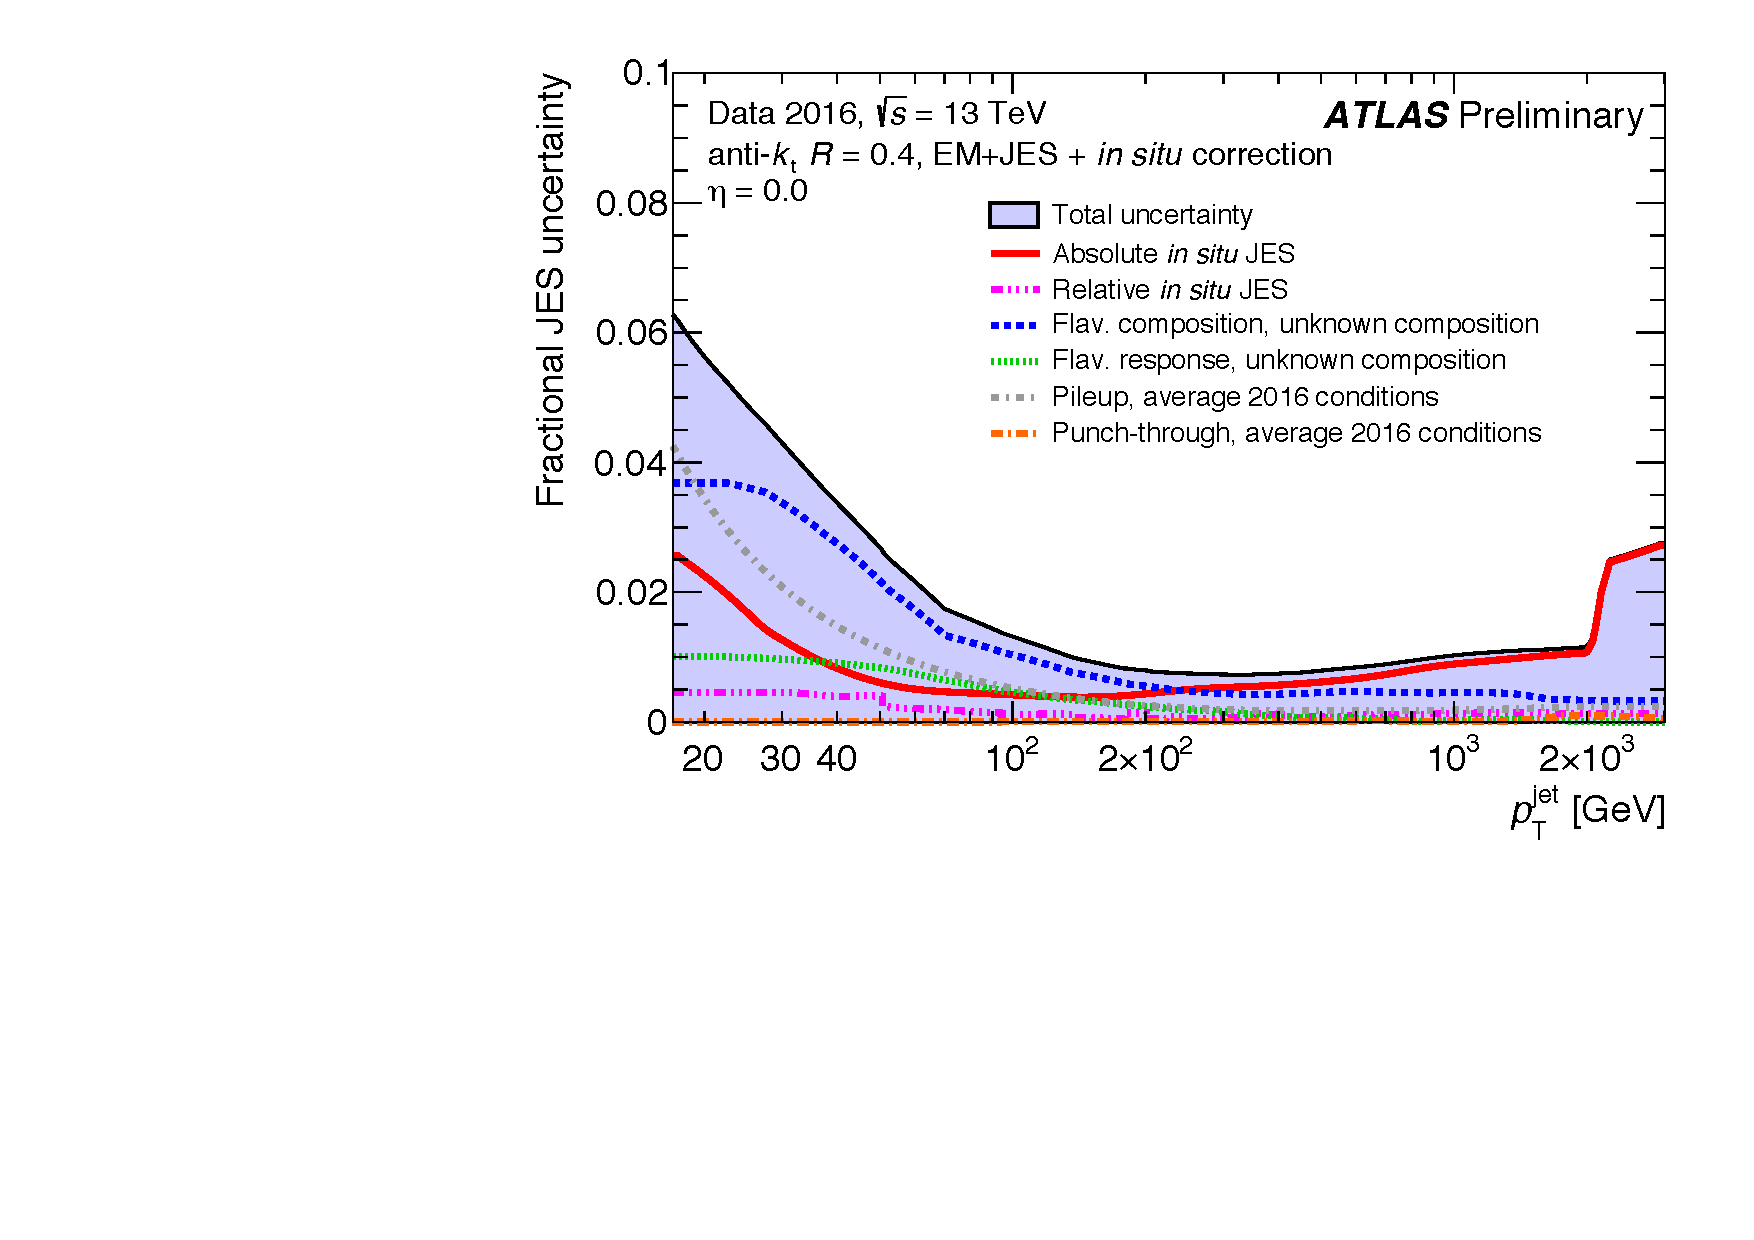
\includegraphics[width=.48\textwidth]{figures/SystematicUncertainties/jes_unc}\label{fig:jes_unc:a}}
\subfloat[]{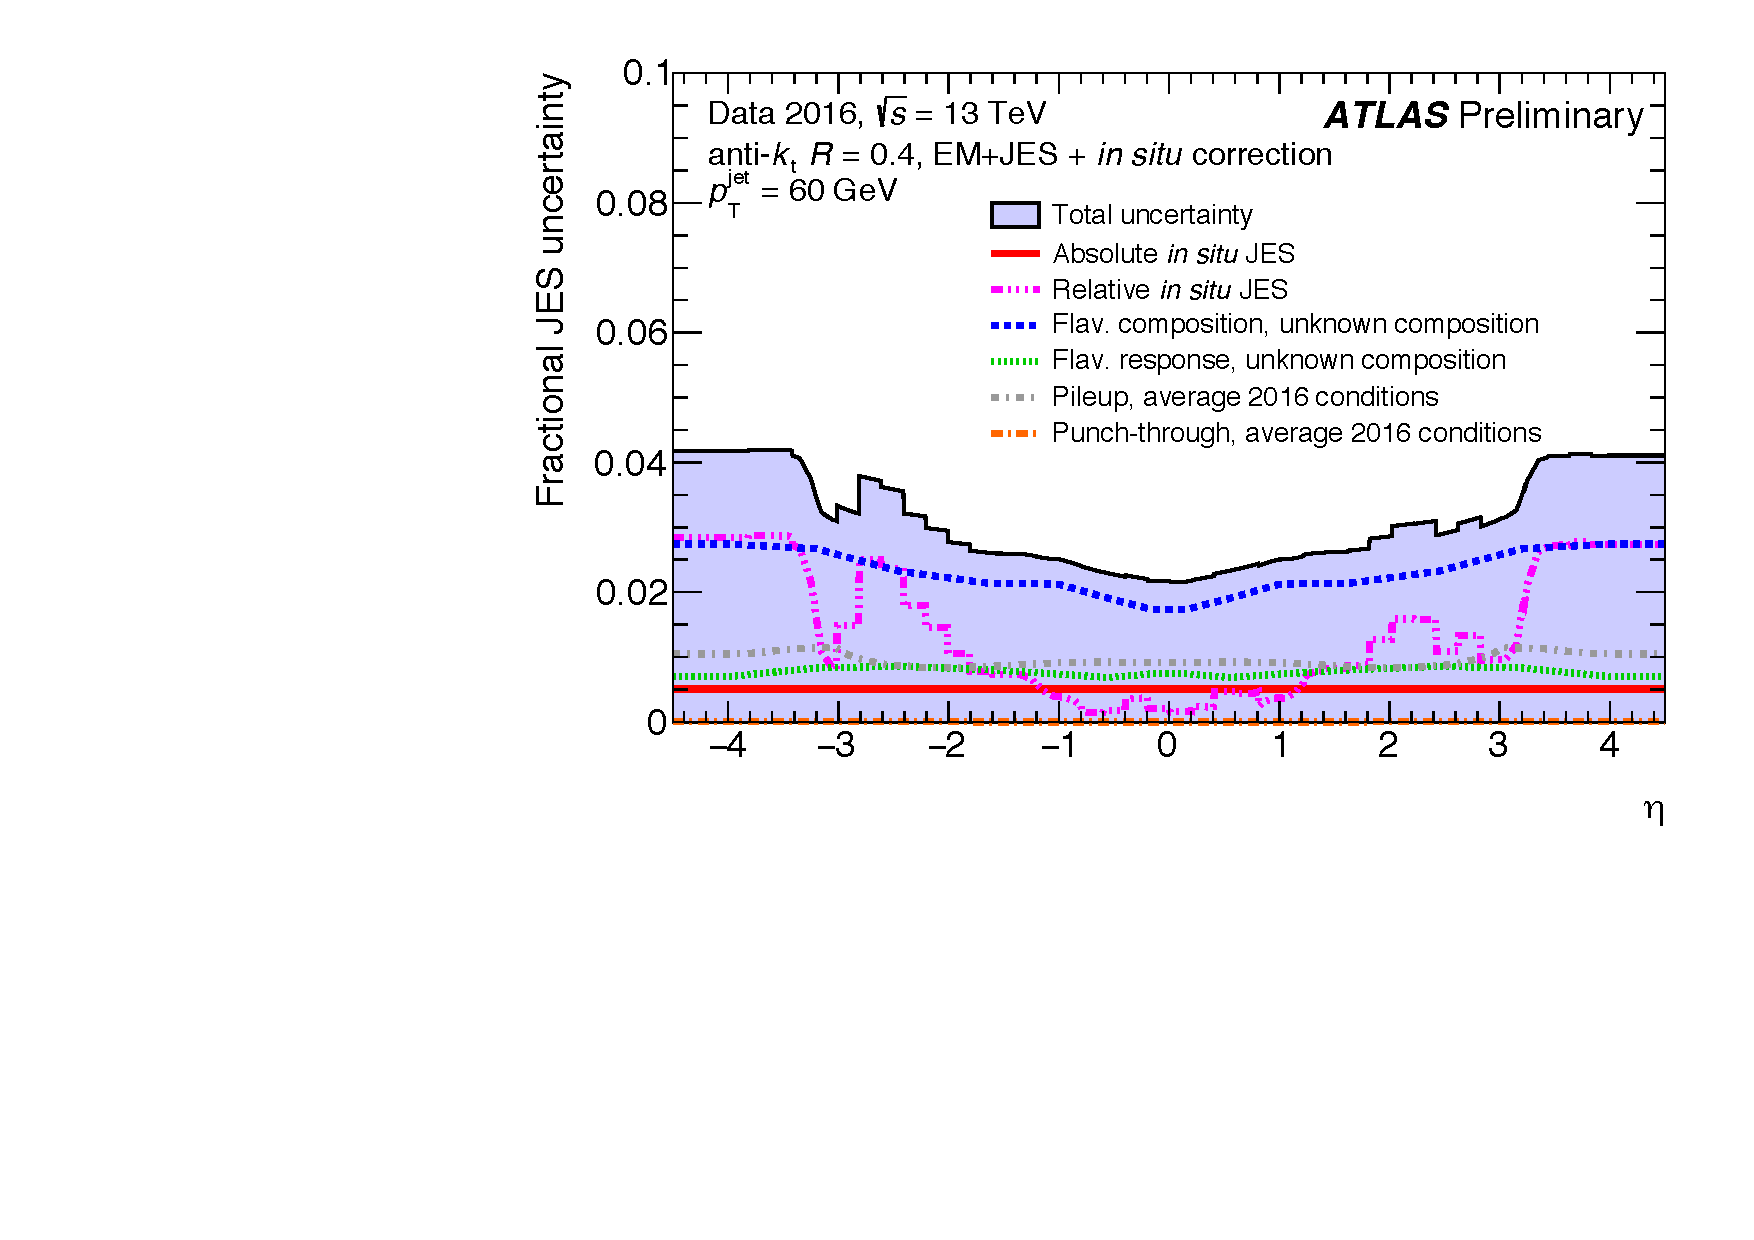
\includegraphics[width=.48\textwidth]{figures/SystematicUncertainties/jes_eta}\label{fig:jes_unc:b}}
\caption[Fractional jet energy scale uncertainty for small-R jets]{The fractional jet energy scale uncertainty for central small-R jets, as a function of \protect\subref{fig:jes_unc:a} \pt (with $\eta=0$) and \protect\subref{fig:jes_unc:b} $\eta$\, (for $\pT=60\,\GeV$)~\cite{jes_unc}.}
\label{fig:jes_unc}
\end{figure}

Uncertainties on $b$-tagging efficiency and misidentification rates for small-R jets are considered~\cite{b_jet, b_jet_opt}. The uncertainties are propagated to the scale factors applied to MC samples using a reduced set of 14 NPs, called the ``medium'' prescription. There are three, four, and five NPs considered for the tagging efficiency of jets from $b$-hadrons, $c$-hadrons, and light flavor quarks, respectively. Additional NPs account for jets with $\pT$ values above the kinematic reach of the calibration sample, and for extrapolating $c$-jet scale factors to \tau-induced jets. % About 5-10\% uncertainty for b-tag jets

%
\subsection{Large-R Jets}
\label{ch:syst:largerjets}
Uncertainties related to the scale of large-R jet $\pT$, mass, and $D_2^{\beta=1}$ are considered~\cite{J_scale_unc}. Several recommended configurations are provided; however, the choice was determined to have a negligible impact on this study. For consistency with similar searches, the ``medium'' configuration is used.  In this prescription, the $\pT$ and mass scale uncertainties are fully correlated, while the $D_2^{\beta=1}$ scale uncertainty is left independent.  Four NPs are considered for both the substructure, and kinematic scale uncertainties (eight total). These account for differences between data and MC, modeling differences between MC generators, tracking uncertainties, and statistical uncertainties. The uncertainties are estimated using the ratio of calorimeter-based to track-assisted-based variables in data and MC. The ratios are evaluated at both the calorimeter jet mass scale, and the track-assisted jet mass scale. The large-R jet scale uncertainties range from approximately $2-5\,\%$, as shown in~\Fig{\ref{fig:J_unc}}.

\begin{figure}[tb]
\centering
\subfloat[]{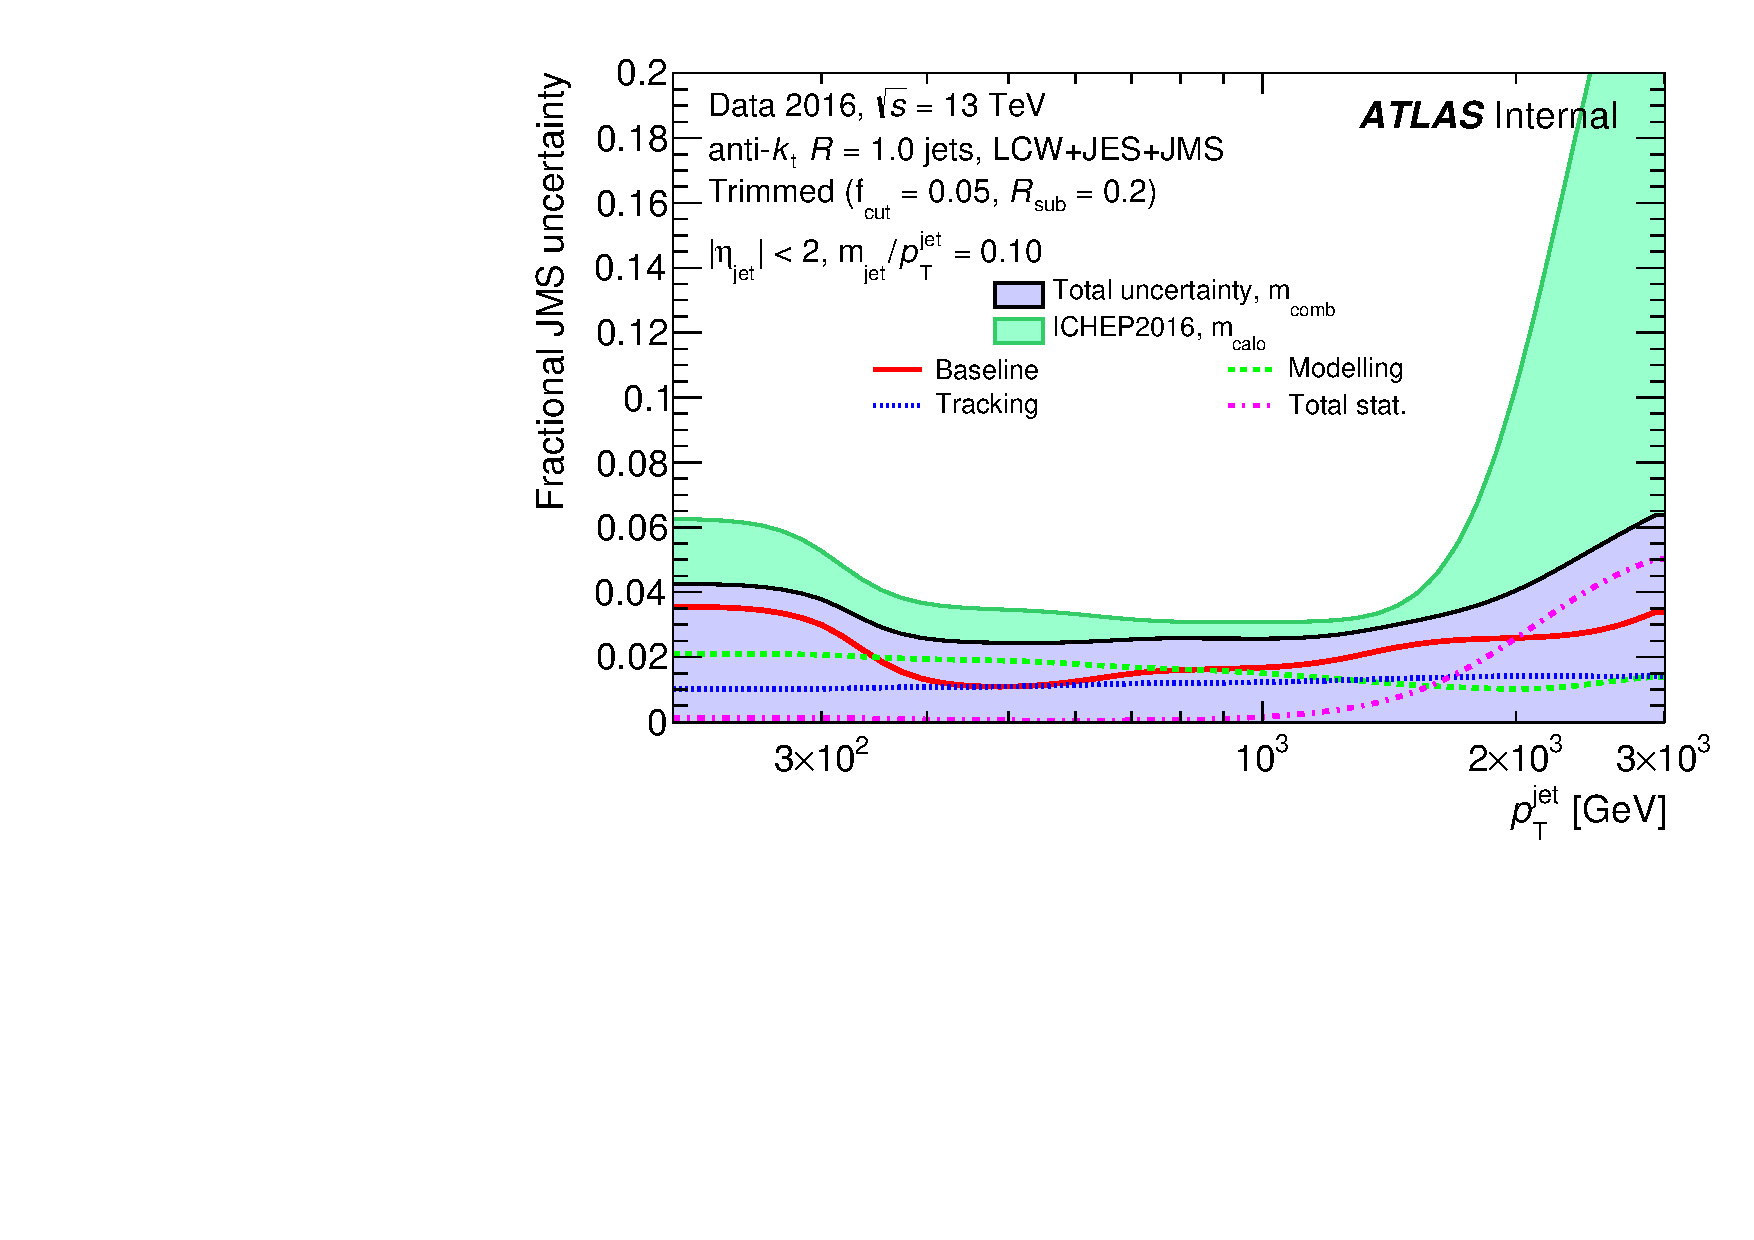
\includegraphics[width=.48\textwidth]{figures/SystematicUncertainties/J_comb_scale}\label{fig:J_unc:a}}
\subfloat[]{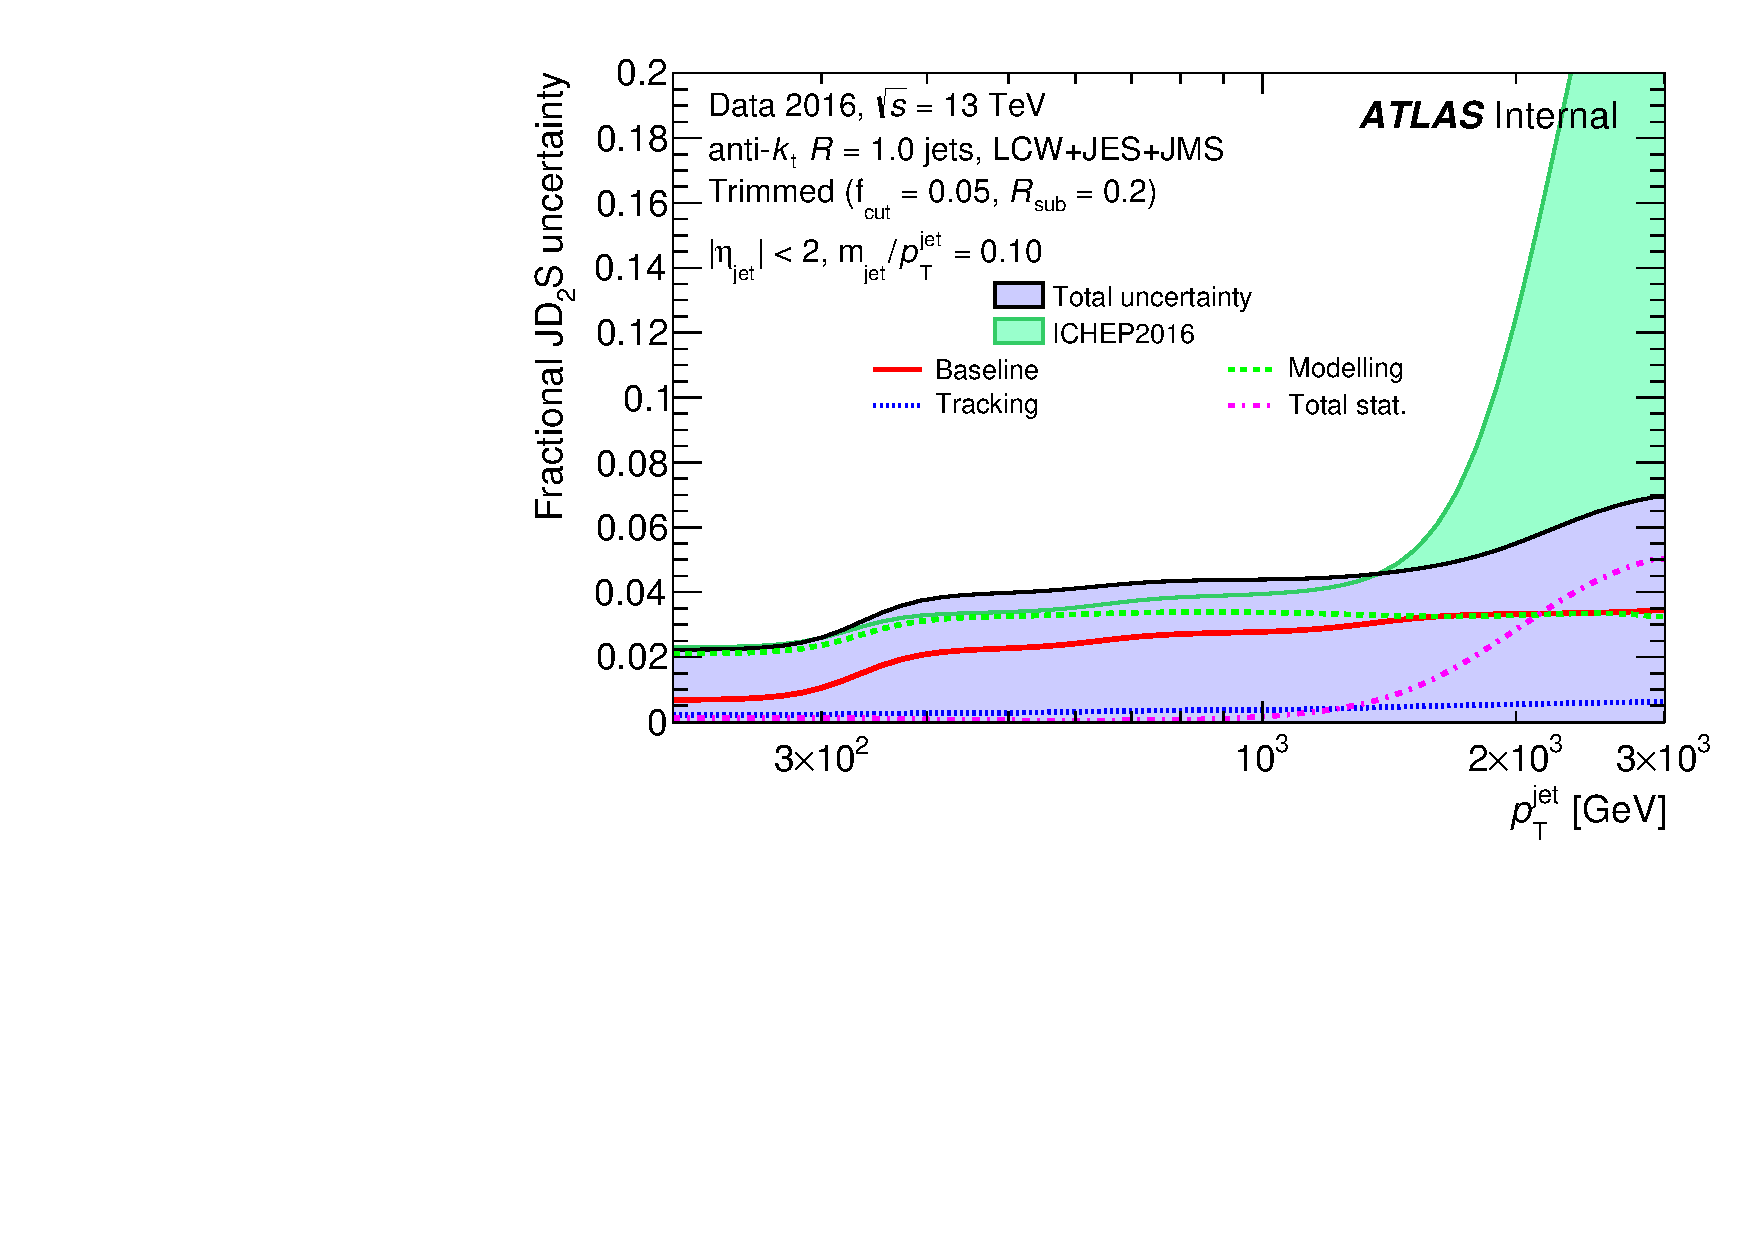
\includegraphics[width=.48\textwidth]{figures/SystematicUncertainties/J_d2_scale}\label{fig:J_unc:b}}
\caption[Fractional scale uncertainty for large-R jet \pT, mass, and $D_2^{\beta=1}$]{The fractional scale uncertainty for large-R jet \protect\subref{fig:J_unc:a} combined mass and \protect\subref{fig:J_unc:b} $D_2^{\beta=1}$, as a function of  \pt. Plots are updated from the procedure used in~\Ref{\cite{jet_comb_mass}}.}
\label{fig:J_unc}
\end{figure}


Resolution uncertainties are applied for large-R jet $\pT$, mass, and $D_2^{\beta=1}$. The recommended procedure is to apply a 2\,\% absolute uncertainty for \pT resolution, and a 20\,\% (15\,\%) relative uncertainty for mass resolution ($D_2^{\beta=1}$ resolution). The absolute uncertainty is applied by smearing the large-R jet \pT with a Gaussian of width, $\sigma=\pT\times2\,\%$. 

The relative uncertainties are applied such that the reconstructed mass ($D_2^{\beta=1}$) has an increased resolution of 20\,\% (15\,\%). First, the MC response of the variable (ratio of reconstructed to truth value) is fit with a Gaussian to extract the width, which gives an estimate of the nominal resolution, $\sigma_{\rm nom}$. The nominal resolution is then smeared with a Gaussian of width $0.66\times\sigma_{\rm nom}$ ($0.57\times\sigma_{\rm nom}$) to increase the measured resolution by 20\,\% (15\,\%)\footnote{
	To increase the resolution by 20\,\%, $(1.2\sigma_{\rm nom})^2 = \sigma_{\rm nom}^2 + (f_{\rm smear}\sigma_{\rm nom})^2$. This corresponds to $f_{\rm smear}=0.66$.
}. The $D_2^{\beta=1}$ response distribution is not approximated well by a Gaussian fit, thus the inter-quartile range is used to estimate the nominal resolution. To be conservative, an additional 2\,\% is added to the smearing value for both the mass and $D_2^{\beta=1}$ resolution. In~\Fig{\ref{fig:larger_res}}, the measured mass and $D_2^{\beta=1}$ resolutions are presented as a function of $\pT$. The $\eta$ dependence, and the difference in resolutions between $W$ and $Z$ jets, were determined to be negligible. Therefore, the smearing is applied only as a function of $\pT$.

\begin{figure}[htb]
\centering
\subfloat[]{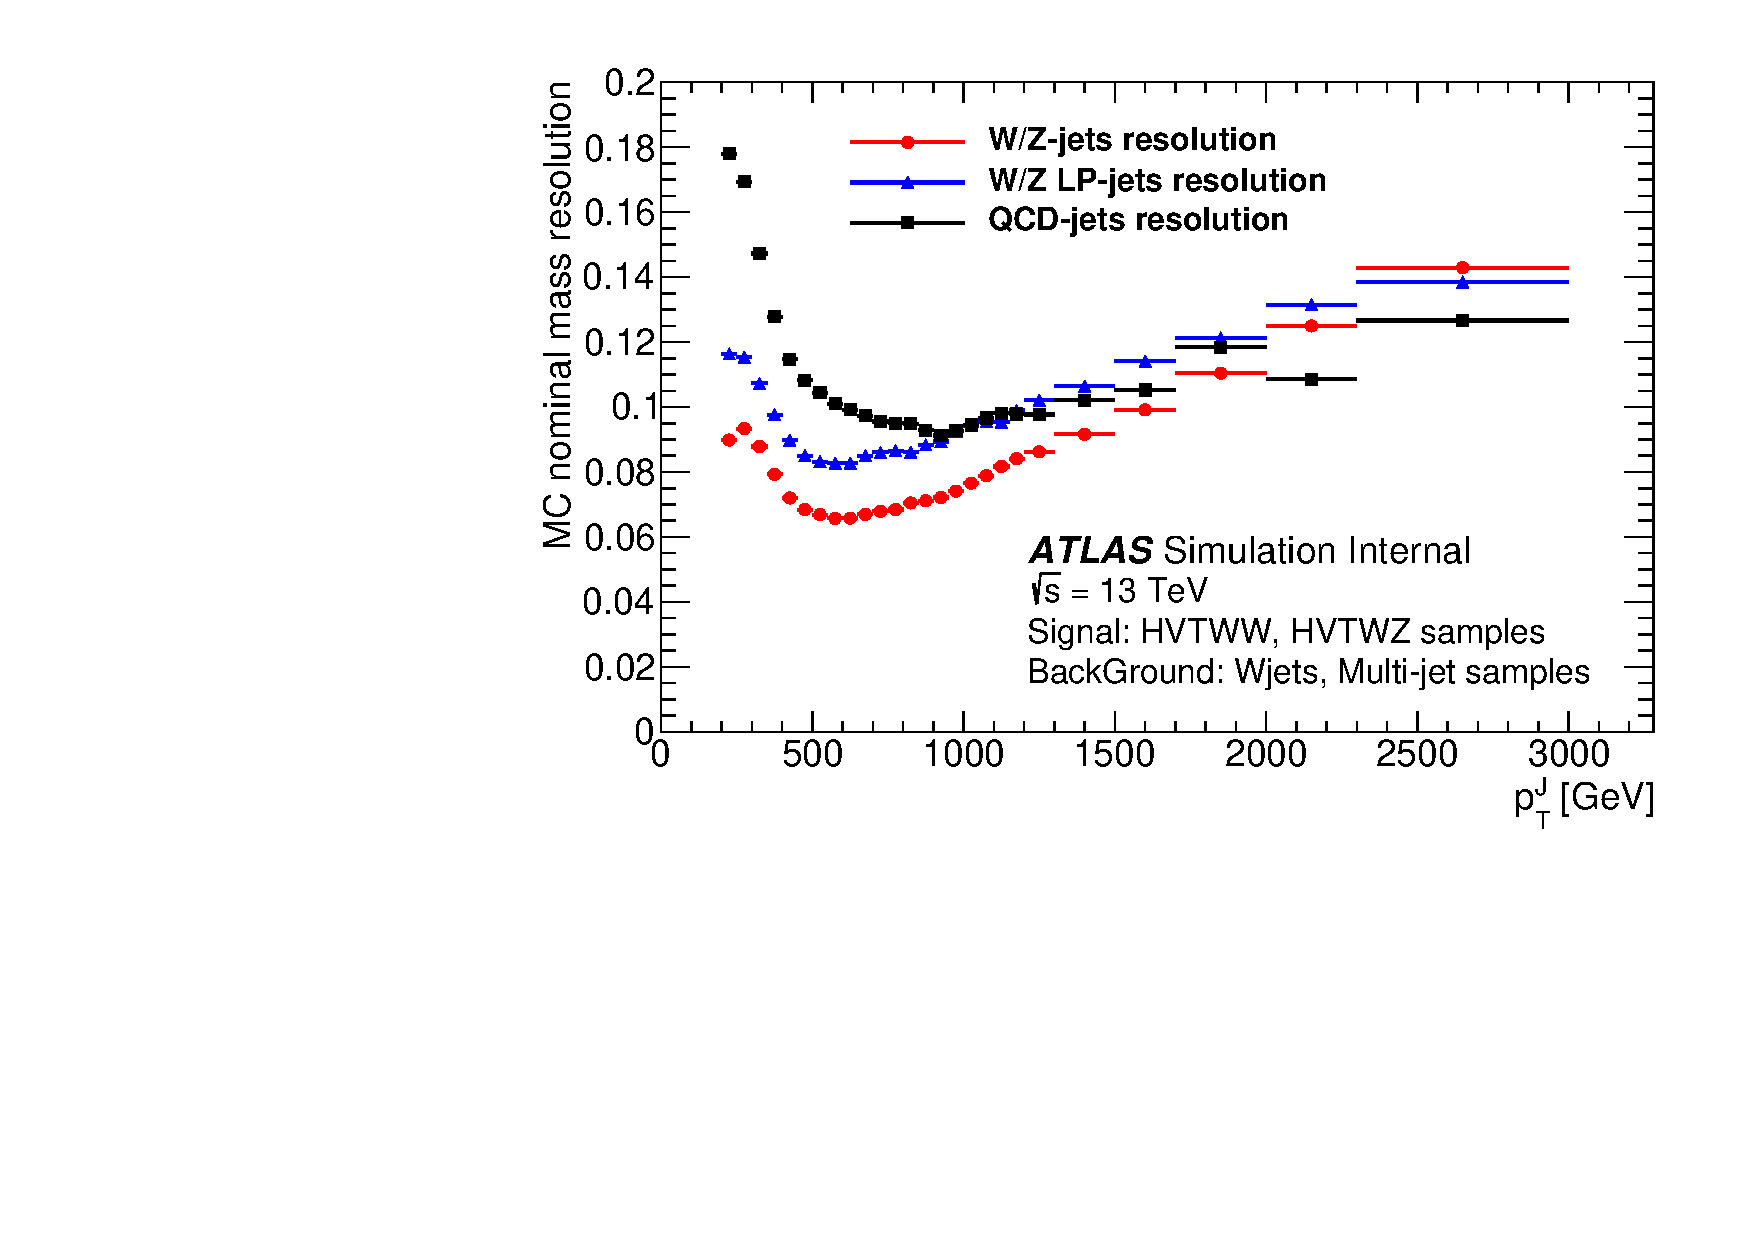
\includegraphics[width=.48\textwidth]{figures/SystematicUncertainties/mass_resolution}\label{fig:larger_res:a}}
\subfloat[]{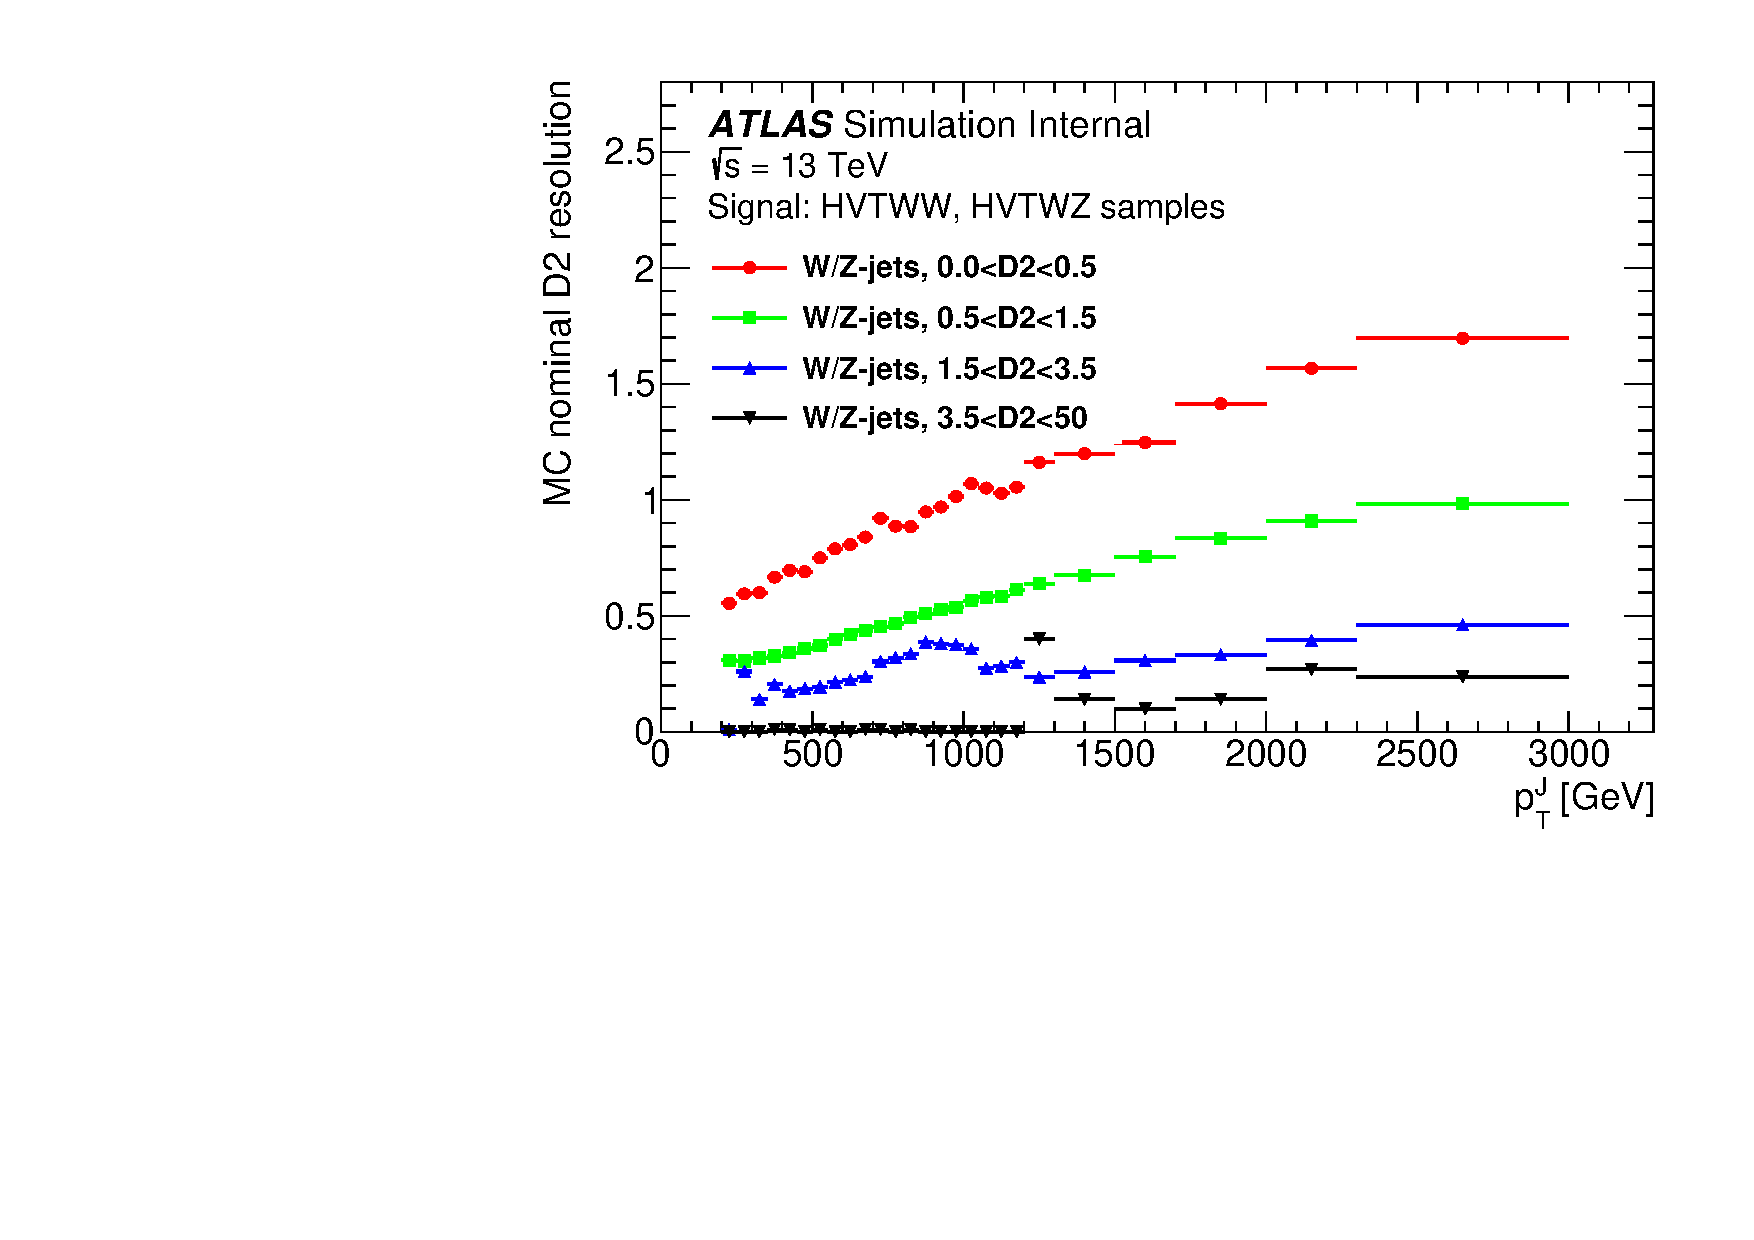
\includegraphics[width=.48\textwidth]{figures/SystematicUncertainties/d2_resolution}\label{fig:larger_res:b}}
\caption[Large-R jet mass and substructure resolution]{The measured large-R jet \protect\subref{fig:larger_res:a} mass resolution and \protect\subref{fig:larger_res:b} $D_2^{\beta=1}$ resolution. The mass resolution is measured separately for high purity and low purity large-R jets. The $D_2^{\beta=1}$ resolution is estimated with the interquartile range (instead of a gaussian fit), resulting in a very conservative uncertainty.}
\label{fig:larger_res}
\end{figure}


%
\subsection{Missing Transverse Energy}
The systematic uncertainties associated with all the reconstructed objects used to build the event \MET are propagated to the reconstructed \MET object, and taken as fully correlated to the uncertainties of the constituent objects. This is the main source of \MET uncertainty. Additional uncertainties are calculated to cover the soft terms in the reconstructed \MET, which involve tracks that are unassociated with any reconstructed object. An uncertainty of approximately 2\,\% is included to cover variations in resolution and scale of the soft term~\cite{met_syst}.


%%
\section{Background Uncertainties}
\label{ch:syst:bkg_unc}
Several systematic uncertainties are included to account for uncertainties in the modeling of the simulated backgrounds. For the two main backgrounds in this search, \Wjets and \ttbar, the normalizations are free to float in the fit (\Ch{\ref{ch:stats}}), and systematics uncertainties are estimated to account for the shape of the $m(\ell\nu J)$ distribution in the SRs.

Both the \Singlet and \Zjets backgrounds contribute a small amount to the total estimated SM background in this search. The shapes for these backgrounds are derived exclusively from the MC prediction. A systematic uncertainty is applied to the normalizations of the \Singlet and \Zjets backgrounds to account for the uncertainty in the SM cross section measurement. The normalizations are allowed to float, with an imposed Gaussian constraint with 11\,\% width.

The SM diboson production cross section is fixed to the inclusive NLO calculation. A systematic uncertainty on the normalization is applied in the same manner as for the \Singlet and \Zjets backgrounds. In this case, the width of the Gaussian constraint is set to 30\,\%, in order to cover both the production cross section uncertainty ($\sim11\,\%$) and the factorization and renormalization scale uncertainty ($\sim20\,\%$). Alternative samples produced with \textsc{Powheg-Box+Pythia} are compared to the nominal \textsc{Sherpa} samples, and used to evaluate any shape modeling uncertainty. The shape difference of the invariant mass distribution between the two MC generators was determined to be negligible. 

%
\subsection{\Wjets Shape Uncertainties}
% Factorization scale: separate hard from soft QCD processes (pert. vs non-pert)
% Renorm scale: Energy scale where you set mu when you renormalize, i.e. top mass etc
% Resummation scale: deal with gluon radiation (otherwise diverges) done at leading log (LL)

Following the recommended procedure, the following modeling variations are considered to estimate the uncertainty in the shape of the \Wjets background:
\begin{itemize}
\item Factorization and renormalization scale variations
\item PDF variations
\item $\alpha_s$ variations
\item CKKW matching scale variations~\cite{ckkw} (for $2\ra n$ processes, how to combine matrix element calculations with parton showering calculations without double counting)
\item Resummation scale variations
\end{itemize}
The corresponding parameters are varied in the nominal generator, \textsc{Sherpa}, to estimate the uncertainty. Additionally, alternative samples generated with \textsc{MadGraph} are compared to the nominal \textsc{Sherpa} samples to estimate systematic uncertainties related to parton showering and matrix element implementations.

For each systematic variation, the normalization is fixed such that the event yield in the \Wjets CR is equal to that of the nominal sample. In each SR, the ratio between the variation and nominal $m(\ell\nu J)$ distribution is calculated on a bin-by-bin basis. A linear fit is applied to the ratio in each SR in order to characterize the uncertainty on the shape modeling from the variation. In~\Fig{\ref{fig:wj_syst}}, the HP \Wjets CR is shown for both the VBF and ggF selection, with the dominant systematic shape uncertainties overlaid.

\begin{figure}[htb]
\centering
\subfloat[]{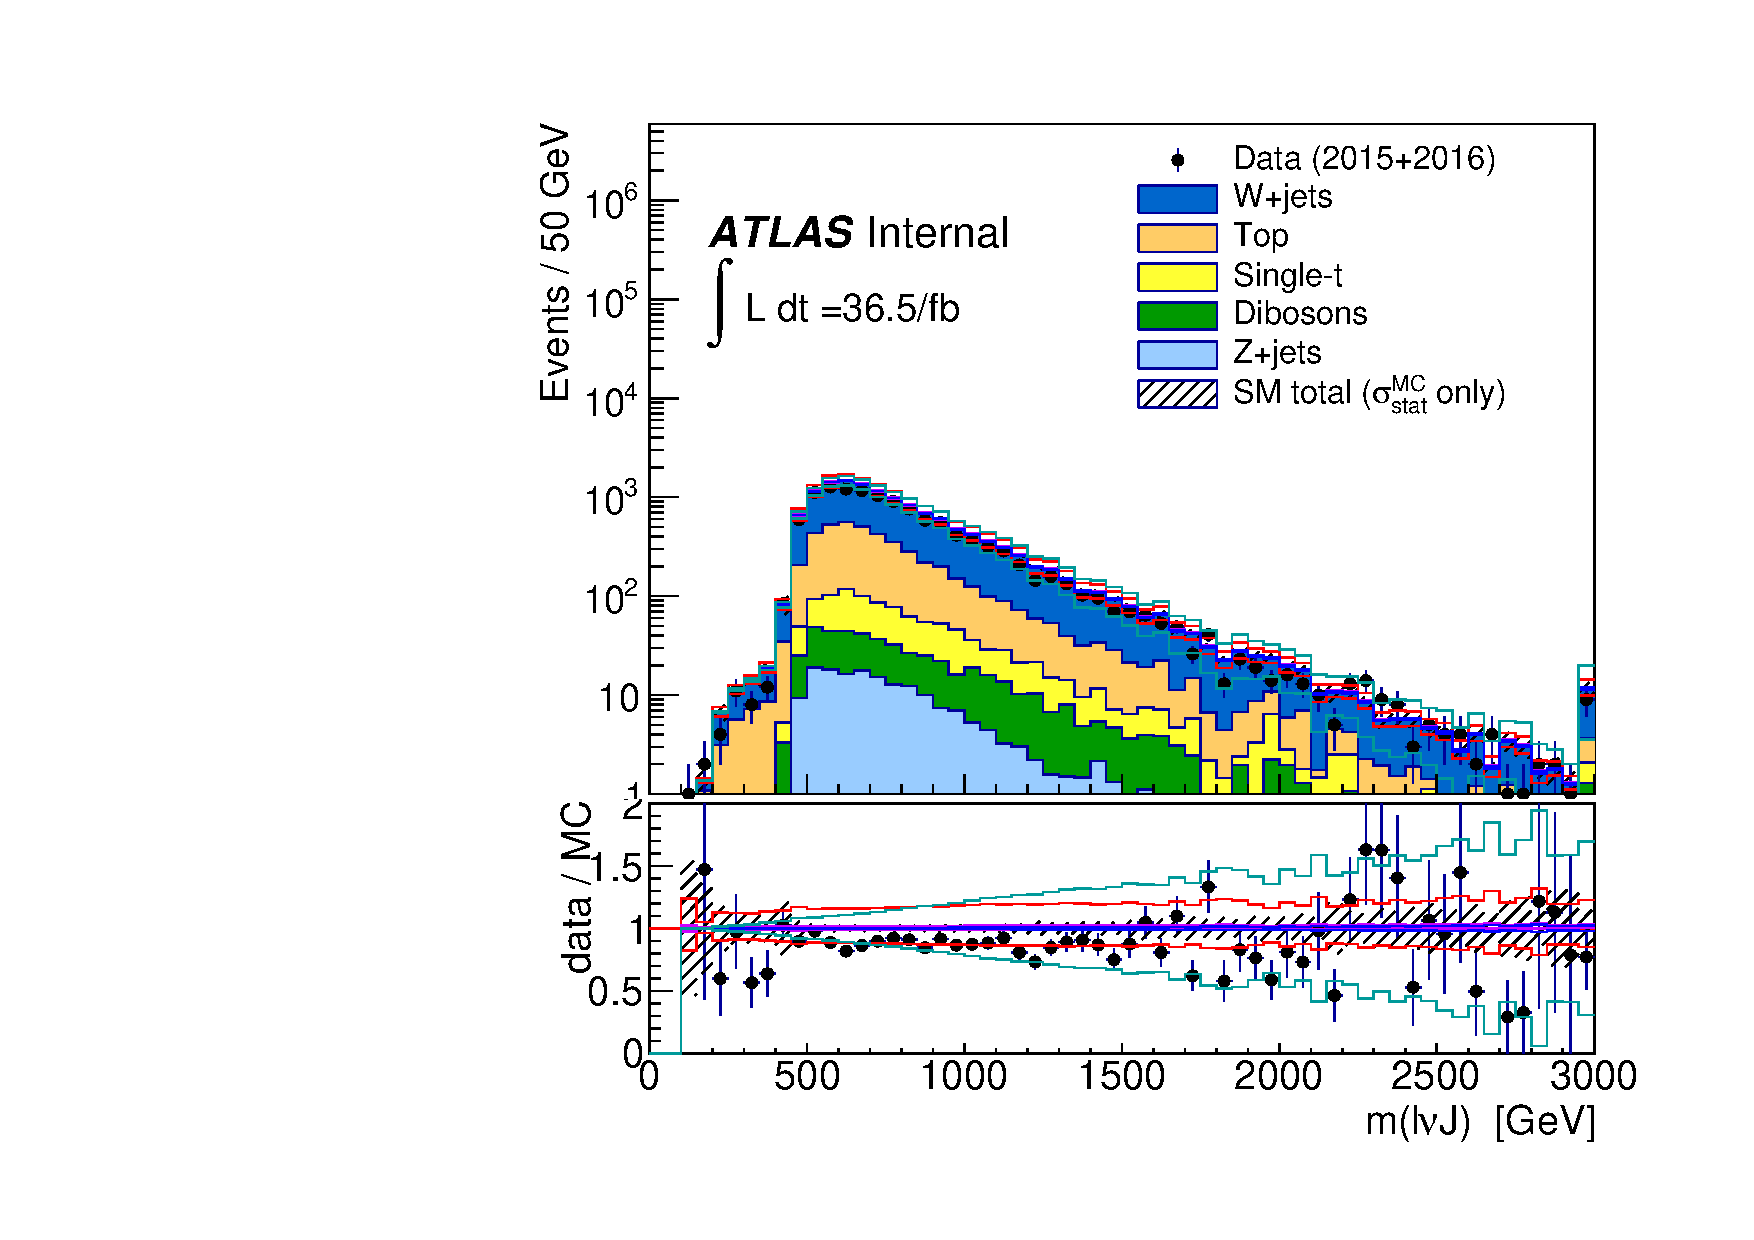
\includegraphics[width=.49\textwidth]{figures/SystematicUncertainties/VVM_CRWHP_ggF}\label{fig:wj_syst:a}}
\subfloat[]{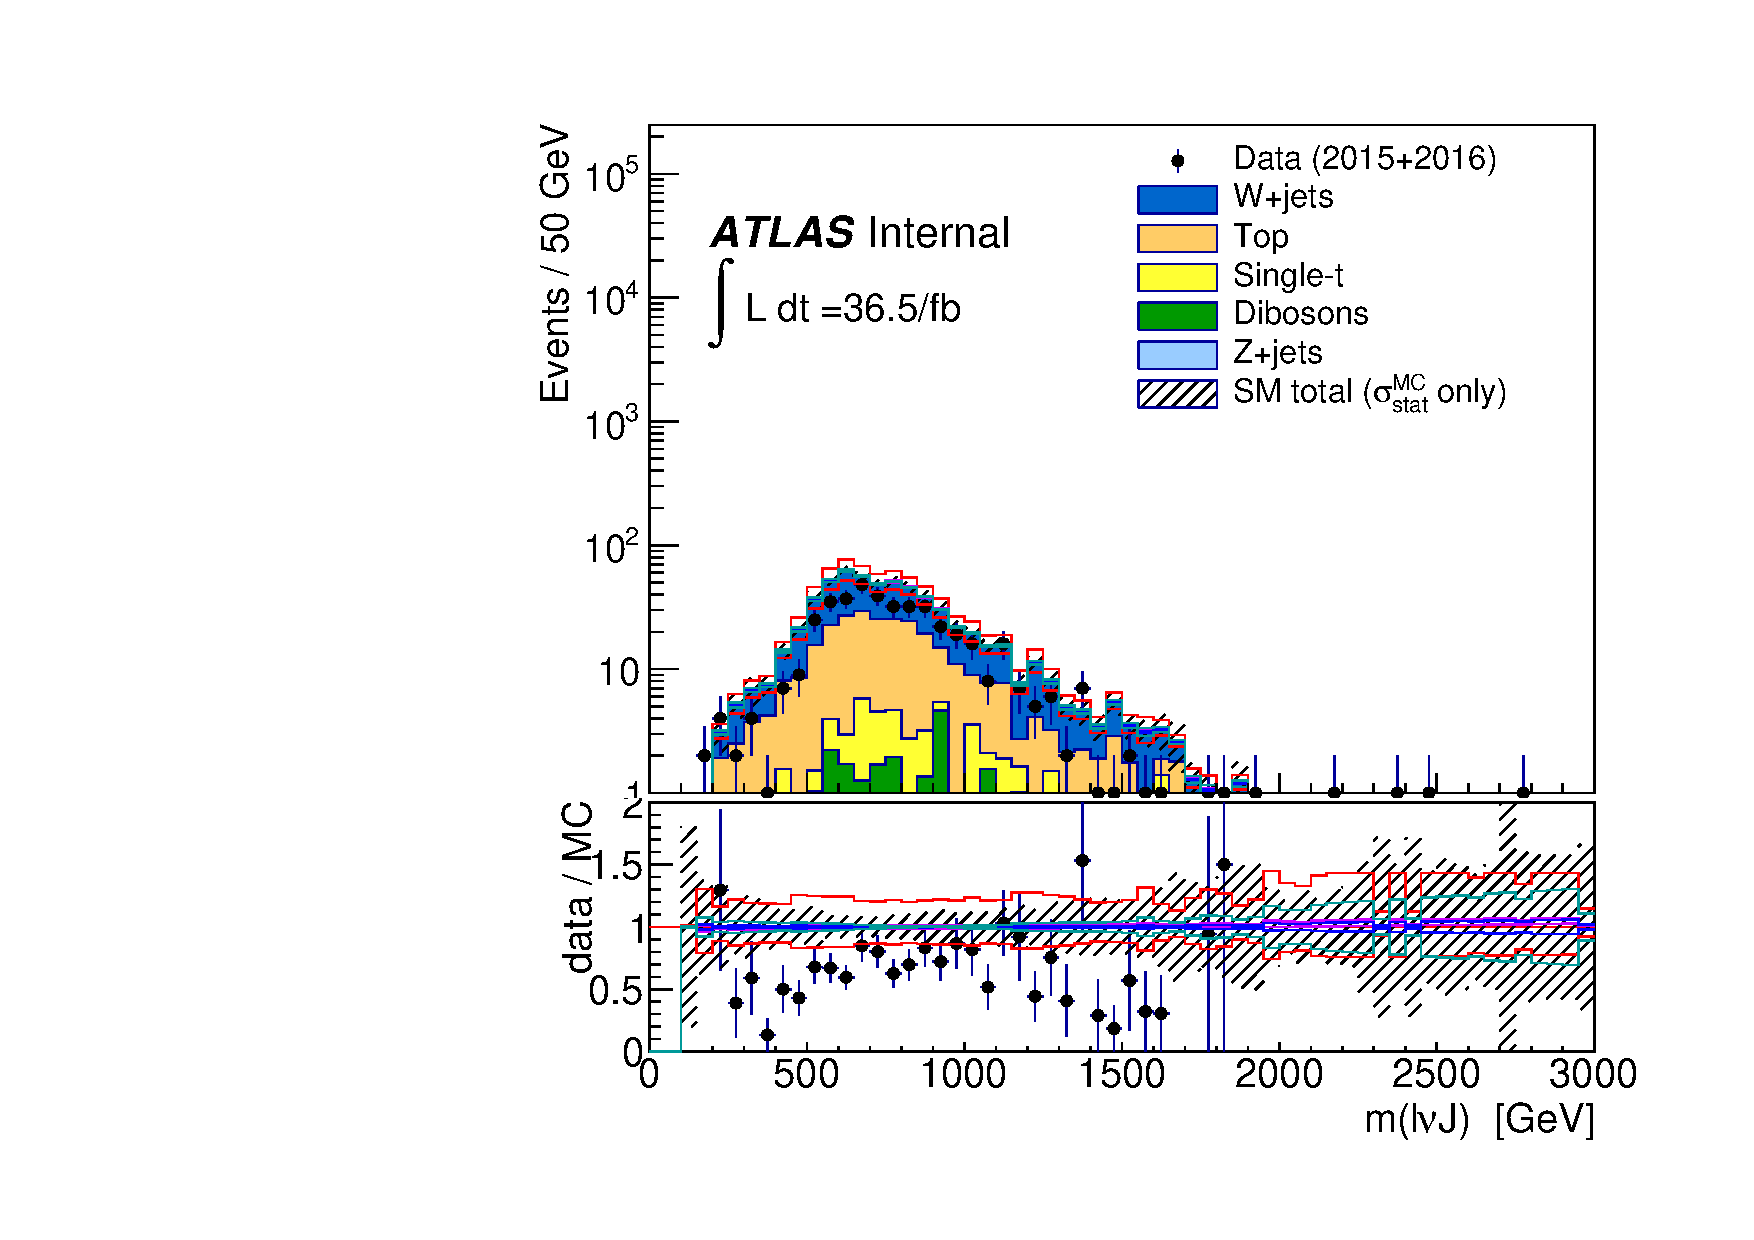
\includegraphics[width=.49\textwidth]{figures/SystematicUncertainties/VVM_CRWHP_VBF}\label{fig:wj_syst:b}}
\caption[\Wjets modeling variations in the \Wjets high purity control region]{The $m(\ell\nu J)$ distribution in the \Wjets CR for \protect\subref{fig:wj_syst:a} ggF selection and \protect\subref{fig:wj_syst:b} VBF selection. Dominant \Wjets modeling uncertainties affecting the shape are shown by colored lines: factorization and renormalization scale variation (red), $\alpha_s$ variation (violet), PDF variation (blue) and \textsc{Sherpa}/\textsc{MadGraph} difference (cyan). The normalization is allowed to float in the final fit described in~\Ch{\ref{ch:stats}}.}
\label{fig:wj_syst}
\end{figure}

%
\subsection{\ttbar Shape Uncertainties}
To estimate the shape uncertainty of the $m(\ell\nu J)$ distribution for the \ttbar background, alternative samples generated with \textsc{MC@NLO} are compared to the nominal samples generated with \textsc{Powheg-Box}. Additional uncertainties related to parton showering are estimated by comparing alternative samples using \textsc{Herwig++} to the nominal samples using \textsc{Pythia}. Renormalization and factorization scale uncertainties are estimated by setting the corresponding parameters in the nominal generator to one half, and to double their nominal values. 

Analogous to the \Wjets procedure, the normalization of the systematic variations are fixed such that the event yield in the \ttbar CR is equal to that of the nominal sample. For each SR, the ratio between the variation and the nominal $m(\ell\nu J)$ distribution is calculated bin-by-bin. Finally, a linear fit is applied to the ratio to estimate the uncertainty on the shape modeling from the variation. 


%%
\section{Signal Uncertainties}
\label{ch:syst:sig_unc}
The largest contributions to the uncertainty on the event yield of the generated signal samples are from initial state and final state radiation (ISR and FSR, respectively), and choice of PDF. 

%
\subsection{Initial State and Final State Radiation Uncertainties}
Following the prescription in~\Ref{\cite{pythia_tune}}, five variations are considered to account for ISR and FSR uncertainties. The variations account for uncertainties related to the underlying event (one), jet substructure (one), and aspects of extra jet production (three). The variations are summed in quadrature and compared to the nominal distribution to estimate the uncertainty. A fourth-order polynomial is fit to the uncertainties, as shown in~\Fig{\ref{fig:isrfsr}}. For most signal models, the estimated uncertainty is approximately 4\,\%.

%
\subsection{Parton Distribution Function Uncertainties}
The uncertainty on the event yield due to choice of PDF is evaluated by comparing samples with the nominal PDF choice, \textsc{NNPDF3.0}, to alternative samples generated with \textsc{MMHT2014}~\cite{mmht} and \textsc{CT14}~\cite{CT14} PDFs\footnote{
	The nominal RS $G^*$ samples are generated with the \textsc{CT14} PDF set, thus the uncertainty is estimated with alternative samples using the \textsc{NNPDF3.0} and \textsc{MMHT2014} PDF sets.
}. Following the prescription in~\Ref{\cite{pdf_env}}, the 68\,\% uncertainty bands for each PDF set are used to evaluate the variations, and the envelope of the three variations is kept to estimate the signal uncertainty. The uncertainty is measured on the ratio of the efficiency times acceptance ($\epsilon\times A$) of the variation samples to the nominal samples. In~\Fig{\ref{fig:pdf}}, the estimated uncertainty due to choice of PDF is shown for the HVT $Z'$ signal model. The estimated uncertainties range among the signal models from approximately $0.5-2.0\,\%$.
\begin{figure}[tb]
\centering
\subfloat[]{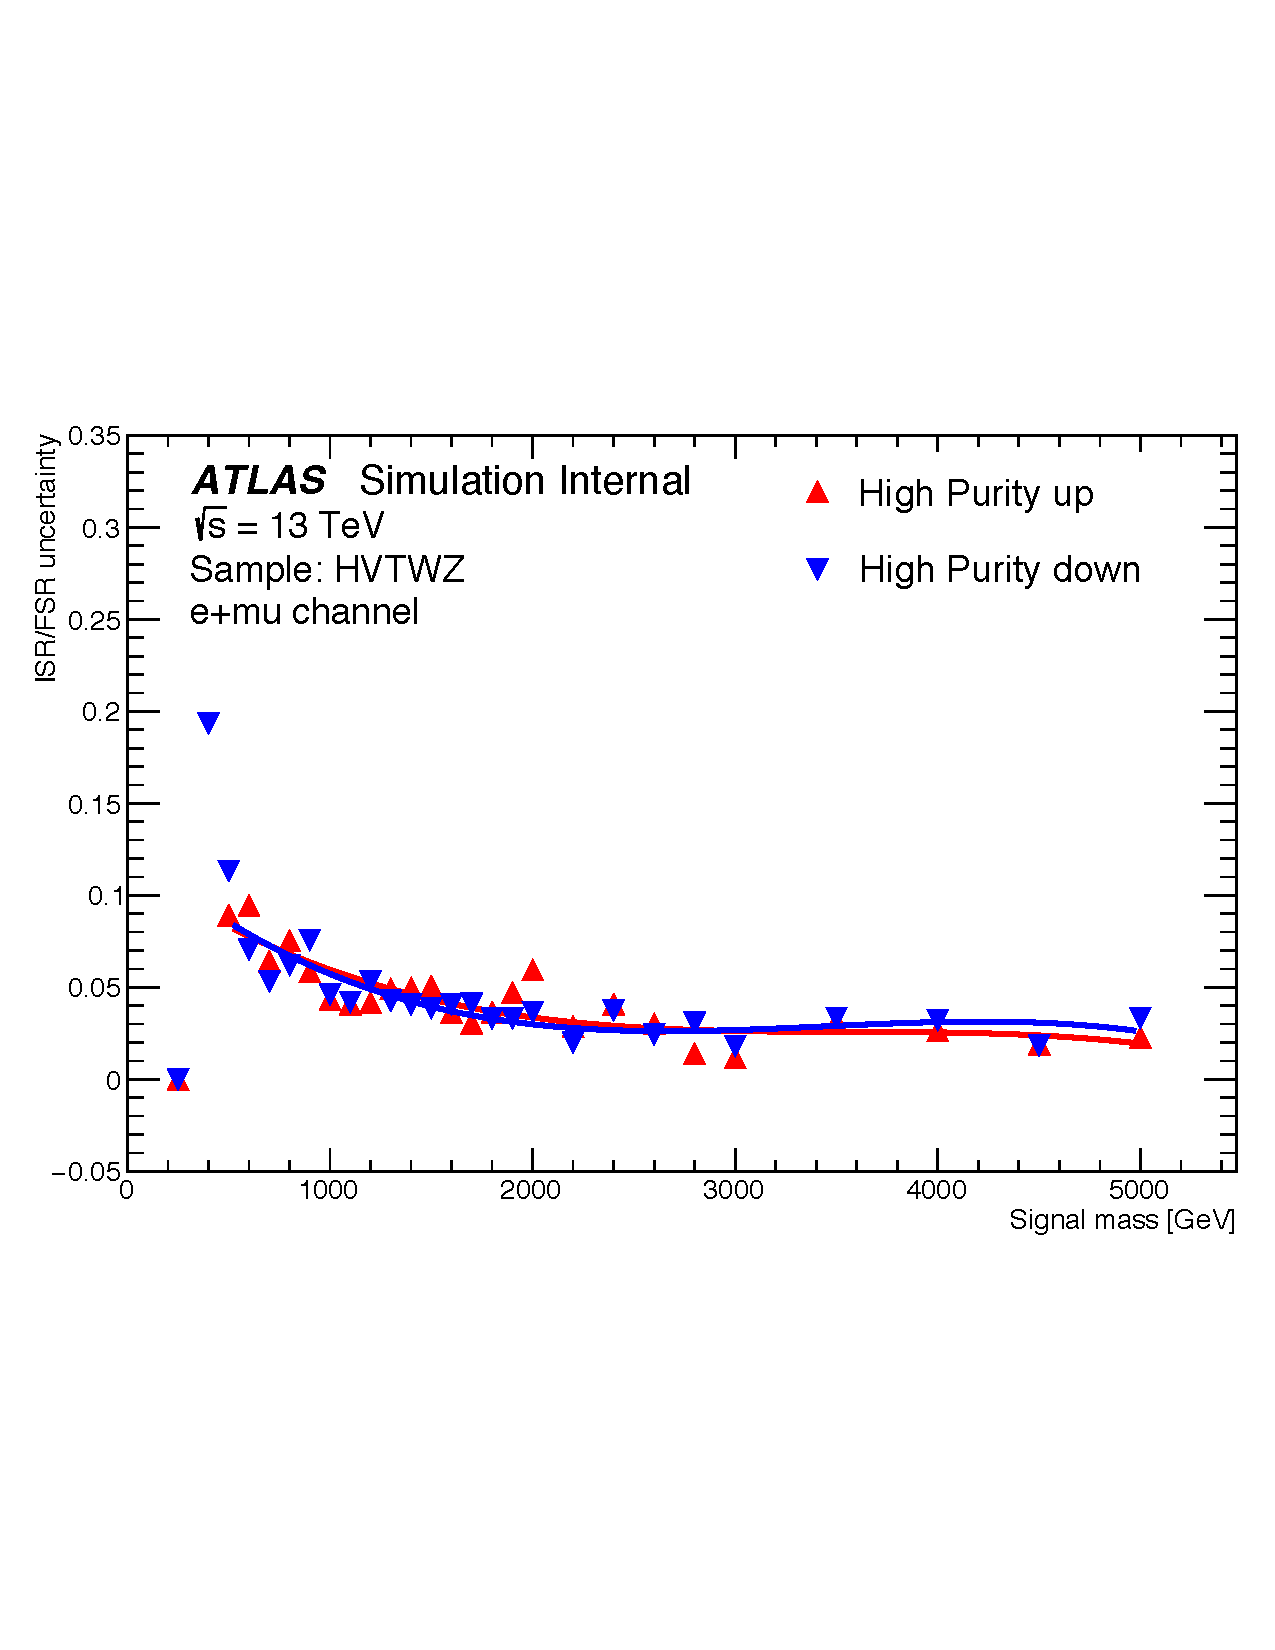
\includegraphics[width=.49\textwidth]{figures/SystematicUncertainties/ISRFSR_HVT3}\label{fig:isrfsr:a}}
\subfloat[]{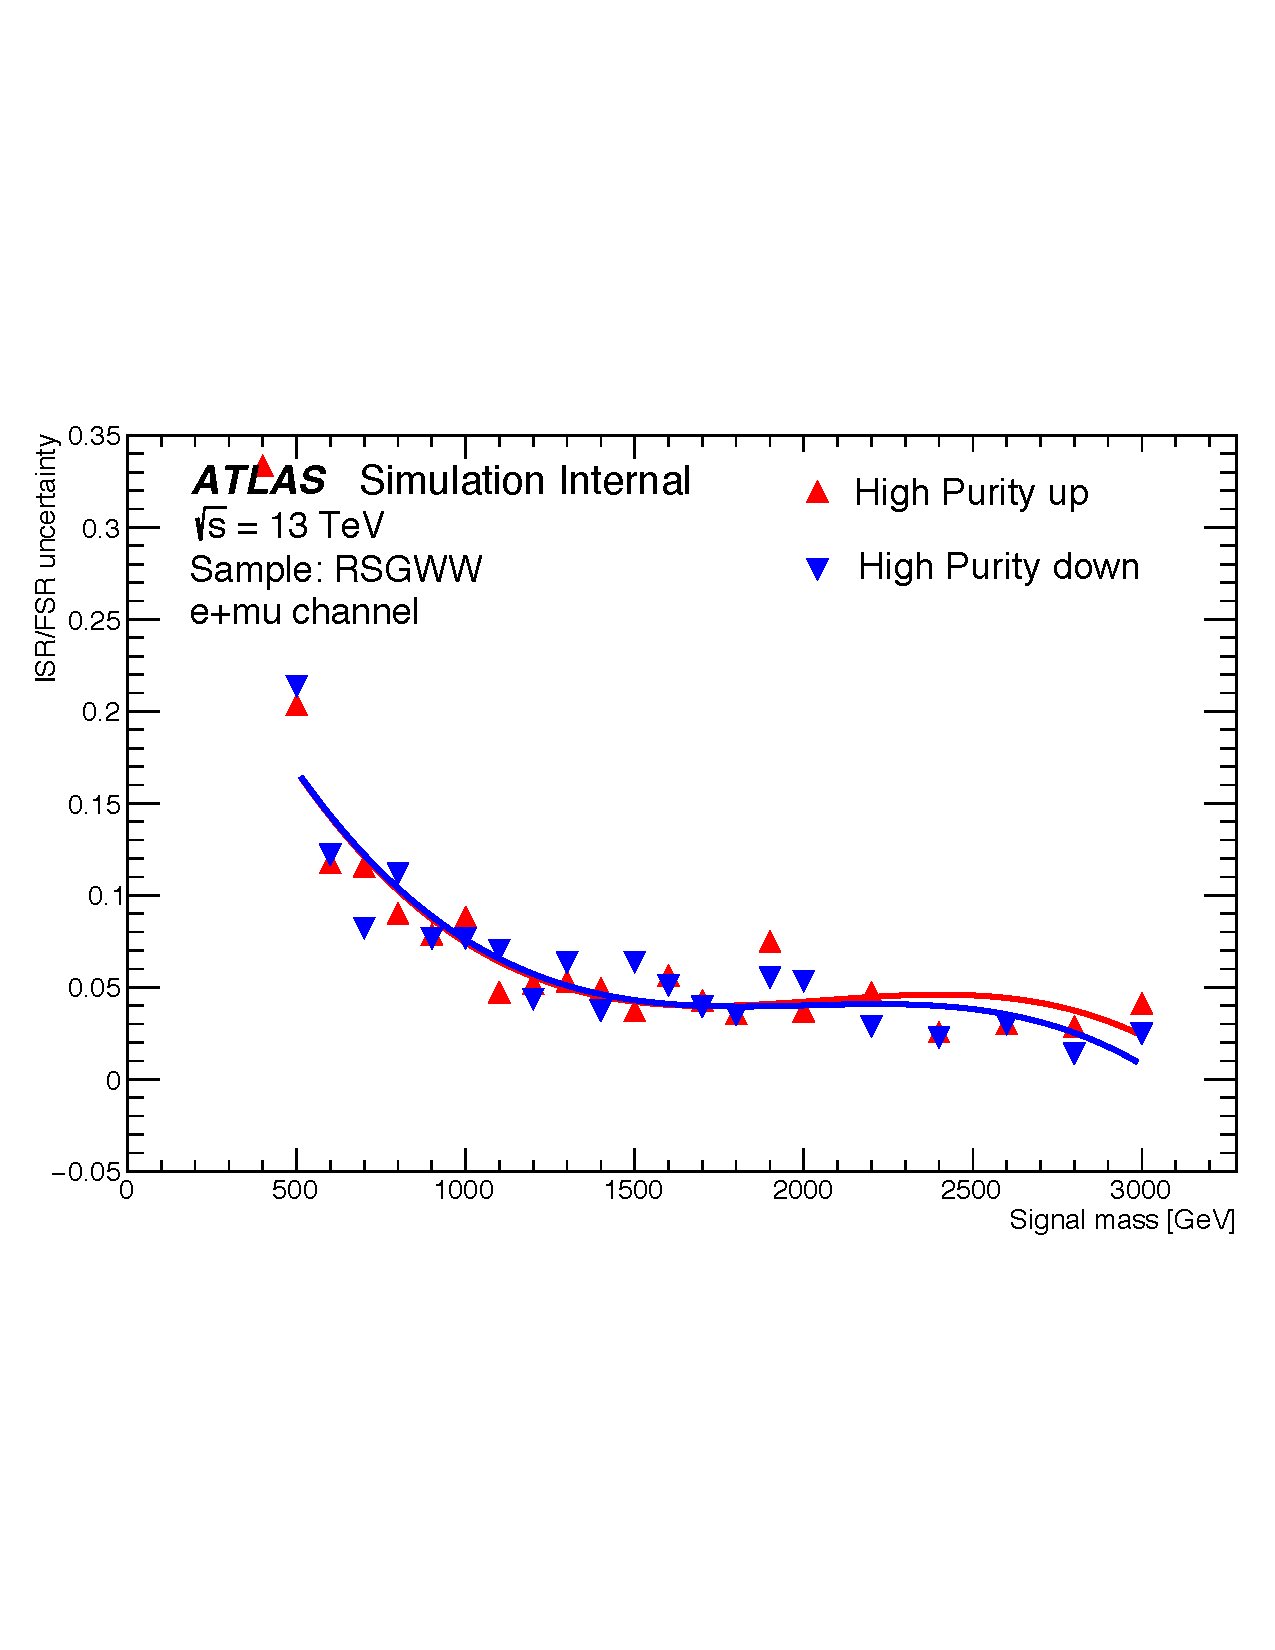
\includegraphics[width=.49\textwidth]{figures/SystematicUncertainties/ISRFSR_RSG3}\label{fig:isrfsr:b}}
\caption[Initial state and final state radiation uncertainties]{Estimated uncertainties related to ISR and FSR in the HP SR for \protect\subref{fig:isrfsr:a} the HVT $W'$ signal model and \protect\subref{fig:isrfsr:b} the RS $G^*$ signal model.}
\label{fig:isrfsr}

\end{figure}
\begin{figure}[htb]
\centering
\subfloat[]{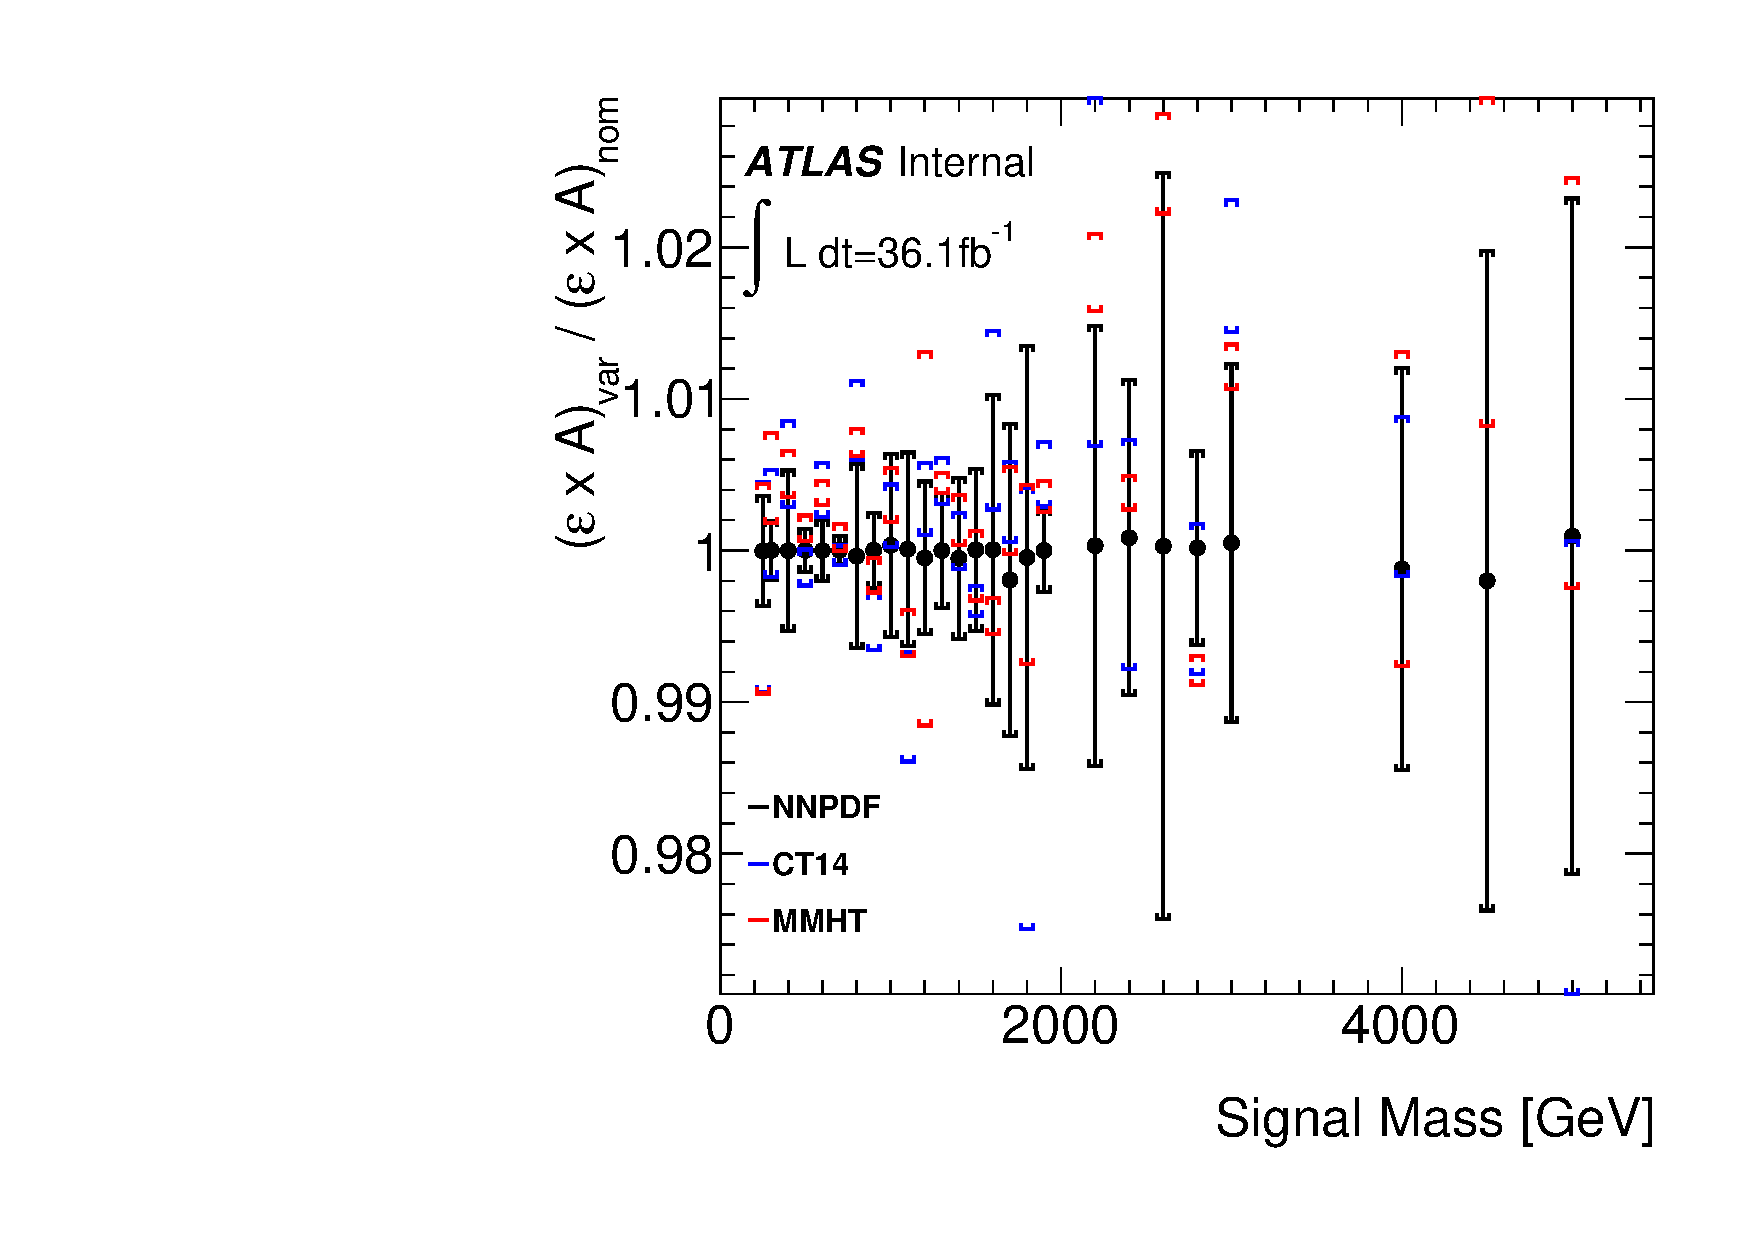
\includegraphics[width=.49\textwidth]{figures/SystematicUncertainties/pdfUncertaintyTotal_HVTWW}\label{fig:pdf:a}}
\subfloat[]{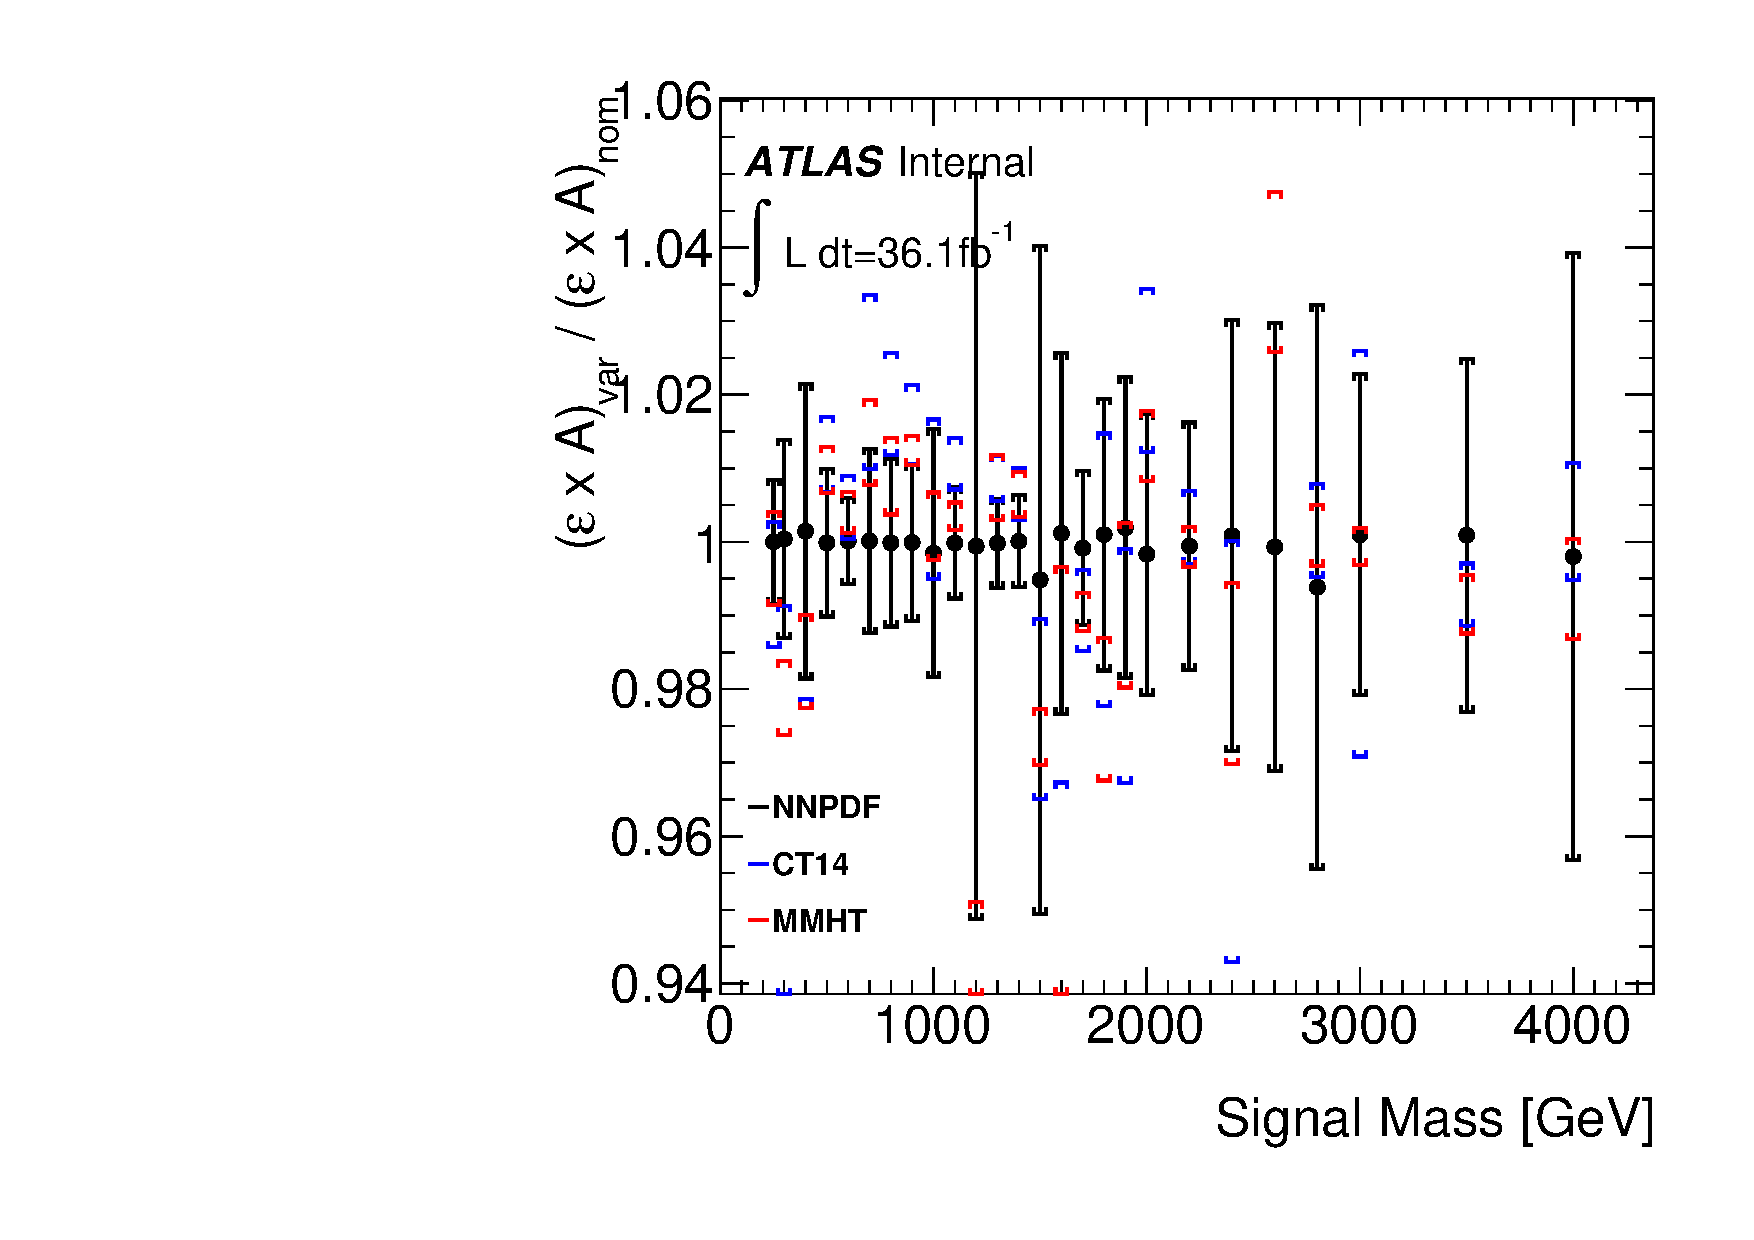
\includegraphics[width=.49\textwidth]{figures/SystematicUncertainties/pdfUncertaintyTotal_HVTWWVBF}\label{fig:pdf:b}}
\caption[Parton distribution function uncertainties]{The estimated PDF uncertainty from \textsc{NNPDF3.0} (black), \textsc{MMHT} (blue), and \textsc{CT14} (red) on the relative signal acceptance for the HVT $Z'$ signal model with \protect\subref{fig:pdf:a} ggF production and \protect\subref{fig:pdf:b} VBF production. The envelope of these variations is chosen as the signal uncertainty.}
\label{fig:pdf}
\end{figure}

